\documentclass[11pt,a4paper]{article}

\usepackage[T1]{fontenc}
\usepackage[utf8]{inputenc}
\usepackage{lmodern}
\usepackage[shorthands=,turkish]{babel}

\usepackage[a4paper,margin=2.3cm]{geometry}
\usepackage{graphicx}
\usepackage{booktabs}
\usepackage{caption}
\usepackage{subcaption}
\usepackage{hyperref}
\usepackage{xcolor}
\usepackage{enumitem}
\usepackage{authblk}
\usepackage{titlesec}
\usepackage{placeins}

\hypersetup{
  colorlinks=true,
  linkcolor=black,
  urlcolor=blue!60!black,
  citecolor=blue!60!black
}

\titleformat{\section}{\large\bfseries}{\thesection}{0.6em}{}
\titleformat{\subsection}{\normalsize\bfseries}{\thesubsection}{0.6em}{}

\setlength{\textfloatsep}{8pt plus 2pt minus 2pt}
\setlength{\floatsep}{8pt plus 2pt minus 2pt}
\setlength{\intextsep}{8pt plus 2pt minus 2pt}
\captionsetup{font=small,labelfont=bf}
\captionsetup[sub]{font=footnotesize}

\title{\textbf{DataMedX Hackathon 2 --- Ön Değerlendirme Raporu}\\[2pt]
       \large Onkoloji Veri Setinde Diyabet Yükü Analizi, Türkçe NLP ve Kanser Türü Sınıflandırması}

\author[1]{Ahmet Erdem Pamuk\thanks{Takım Kaptanı, \texttt{ahmeterdempmkk@gmail.com}}}
\author[2]{Hamit Tuğrul Arslan}
\author[3]{Ömer Kay}

\affil[1]{Mustafa Hakan Güvençer Fen Lisesi, Ankara}
\affil[2]{İstanbul Teknik Üniversitesi Mesleki ve Teknik Anadolu Lisesi, İstanbul}
\affil[3]{Özel Çağdaş Eğitim Anadolu Lisesi, İzmir}

\date{Takım: \textbf{CatBoost Baseline} \\[2pt] Nisan 2026}

\begin{document}
\maketitle

\begin{abstract}
\noindent
Bu çalışma, İstinye Üniversitesi tarafından düzenlenen DataMedX Hackathon~2 ön değerlendirme görevi kapsamında \textbf{CatBoost Baseline} takımı tarafından hazırlanmıştır. Beş farklı kanser türünden (karaciğer, meme, multipl miyelom, over, prostat) toplam 500 hastayı içeren ve hem laboratuvar değerleri hem de Türkçe epikriz metinleri barındıran veri seti üzerinde üç yönlü bir analiz gerçekleştirilmiştir: (i) HbA1c değerleri üzerinden ADA eşiklerine göre diyabet/prediyabet yükünün kanser türlerine göre dağılımı, (ii) epikriz metninden TF-IDF ile anahtar terim ve regex tabanlı semptom çıkarımı, (iii) yalnızca rutin laboratuvar ve demografik özelliklerle eğitilen iki temel makine öğrenmesi modeli (Lojistik Regresyon ve Rastgele Orman). Ki-kare testi, kanser türleri arasında HbA1c kategorilerinde istatistiksel olarak anlamlı bir fark bulunduğunu ($\chi^2{=}17.03$,~$p{=}0.030$) göstermiştir. Rastgele Orman modeli, $5$-katlı çapraz doğrulamada $\%71.2$ doğruluk elde etmiş; bu, beş sınıflı görevde rastgele tahminin (\%20) yaklaşık $3.5$~katıdır. Tüm kod tabanı; her bir adım için ayrı ve \emph{conventional commit} mesajlarıyla GitHub üzerinde yayımlanmıştır.
\end{abstract}

\section{Giriş ve Problem Tanımı}

DataMedX Hackathon~2 ön değerlendirme aşamasında bizden, paylaşılan veri seti üzerinde onkoloji, görüntü işleme veya doğal dil işleme alanlarından bir veya birkaçına yönelik basit bir uygulama, veri analizi ya da model önerisi geliştirmemiz beklenmiştir. Veri seti incelendiğinde; başlığın aksine yalnızca diyabet odaklı değil, \textbf{onkoloji ve diyabetin kesişiminde} yer alan, içinde HbA1c ölçümlerinin yanında klasik onkolojik laboratuvar paneli ve Türkçe epikriz metinleri bulunan zengin bir kaynakla karşılaştığımızı tespit ettik. Bu nedenle çalışmamızı tek bir alana sıkıştırmak yerine üç tamamlayıcı eksende kurguladık:

\begin{enumerate}[leftmargin=1.5em,itemsep=2pt]
    \item \textbf{Klinik analiz:} Kanser türlerine göre diyabet ve prediyabet yükünün karşılaştırılması.
    \item \textbf{Doğal dil işleme:} Türkçe epikriz metinlerinden anahtar terim ve semptom çıkarımı.
    \item \textbf{Makine öğrenmesi:} Yalnızca rutin laboratuvar değerleri kullanılarak kanser türünün tahmin edilmesi.
\end{enumerate}

Görev, \emph{basit ama anlamlı} bir uygulama üretmek olarak tanımlanmıştır; bu çerçevede derin öğrenme veya hiper-parametre optimizasyonu gibi karmaşıklık katacak yaklaşımlardan bilinçli olarak kaçınılmış, açıklanabilir ve klinik olarak yorumlanabilir baseline'lar tercih edilmiştir.

\section{Veri Seti}

Veri seti, \texttt{datamedx\_veriset\_26.xlsx} dosyasında yer almakta; $500$ satır ve $54$ sütundan oluşmaktadır. Her bir kanser türünden $100$ hasta bulunmakta, dolayısıyla sınıflar arasında mükemmel denge sağlanmaktadır. Tablo~\ref{tab:dataset} veri setinin temel istatistiklerini özetlemektedir.

\begin{table}[htbp]
\centering
\caption{Veri seti özet istatistikleri.}
\label{tab:dataset}
\small
\begin{tabular}{lr}
\toprule
\textbf{Özellik} & \textbf{Değer} \\
\midrule
Toplam hasta sayısı & 500 \\
Sütun sayısı & 54 \\
Kanser türü sayısı & 5 (her biri 100 hasta) \\
Kadın / Erkek & 291 / 209 \\
Yaş ortalaması (medyan) & 67.2 (69.0) \\
Lab parametre sayısı & 17 \\
HbA1c ölçümü mevcut & 401 / 500 (\%80.2) \\
Epikriz metni mevcut & 500 / 500 (\%100) \\
\bottomrule
\end{tabular}
\end{table}

Veri setinin önemli bir özelliği, hücrelerin büyük bölümünün \texttt{[değer1], [değer2], $\ldots$} biçiminde çoklu zaman noktası içermesidir. Bu yapı, her hasta için aynı laboratuvar testinin farklı tarihlerde tekrarlandığı bir uzunlamasına izlemi temsil etmektedir. Bu nedenle ön işleme aşamasında, köşeli parantez içindeki tüm sayısal değerleri çıkaran, ortalama (\texttt{\_mean}), son değer (\texttt{\_last}) ve ölçüm sayısı (\texttt{\_n}) özetlerini üreten bir \emph{parser} katmanı geliştirilmiştir (\texttt{src/parse\_utils.py}).

Diğer ön işleme adımları:
\begin{itemize}[leftmargin=1.5em,itemsep=1pt]
    \item \texttt{cinsiyet} sütunundan \texttt{[kadın]/[erkek]} etiketleri ayrıştırıldı.
    \item Yaş, $2026 - \texttt{doğum yılı}$ formülüyle hesaplandı.
    \item Epikriz metnindeki \texttt{\_x000D\_} kaçış karakterleri ve fazla boşluklar temizlendi, küçük harfe çevrildi.
    \item \texttt{ölüm durumu} sütunu tamamen boş olduğundan analiz dışı bırakıldı.
\end{itemize}

\FloatBarrier
\section{Keşifsel Veri Analizi (EDA)}

EDA aşamasında demografik dağılım, eksik değer haritası ve kilit laboratuvar değerlerinin kanser türlerine göre dağılımı incelenmiştir (Şekil~\ref{fig:eda}).

\begin{figure}[htbp]
\centering
\begin{subfigure}[t]{0.46\textwidth}
    \centering
    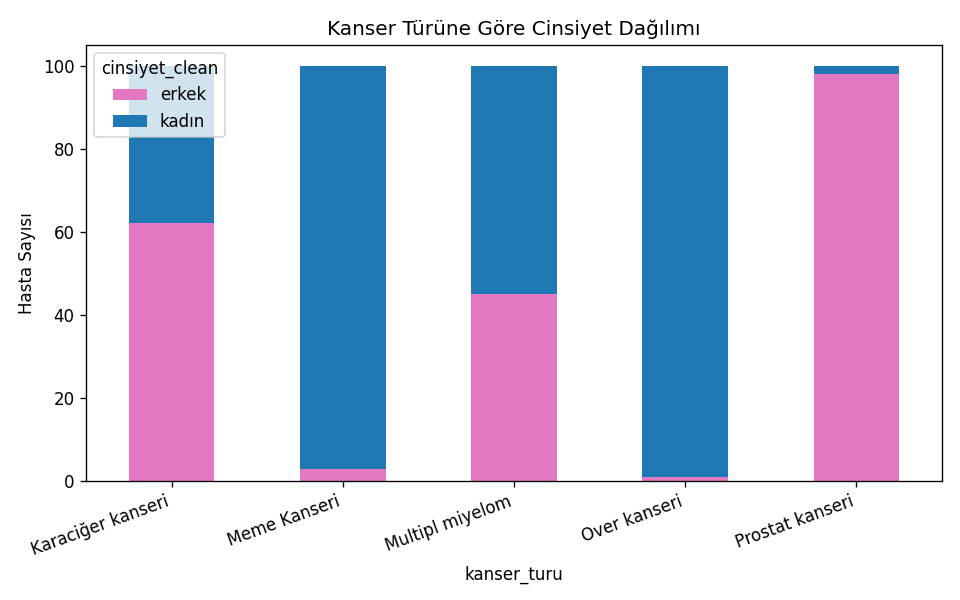
\includegraphics[width=7cm]{../figures/01_gender_by_cancer.png}
    \caption{Cinsiyet dağılımı.}
\end{subfigure}\hfill
\begin{subfigure}[t]{0.46\textwidth}
    \centering
    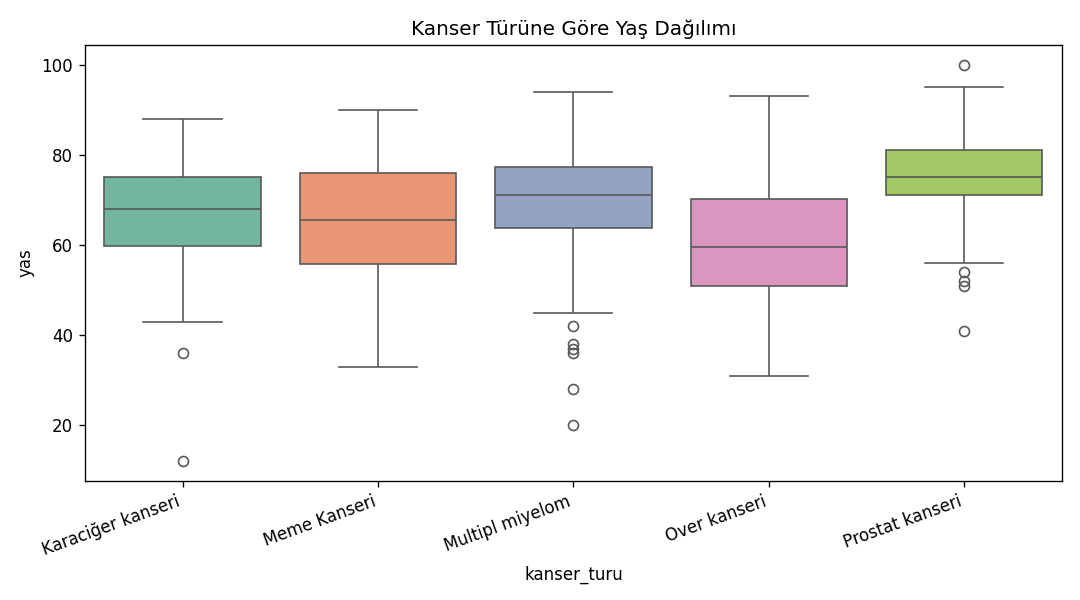
\includegraphics[width=7cm]{../figures/02_age_by_cancer.png}
    \caption{Yaş dağılımı.}
\end{subfigure}

\vspace{6pt}

\begin{subfigure}[t]{0.46\textwidth}
    \centering
    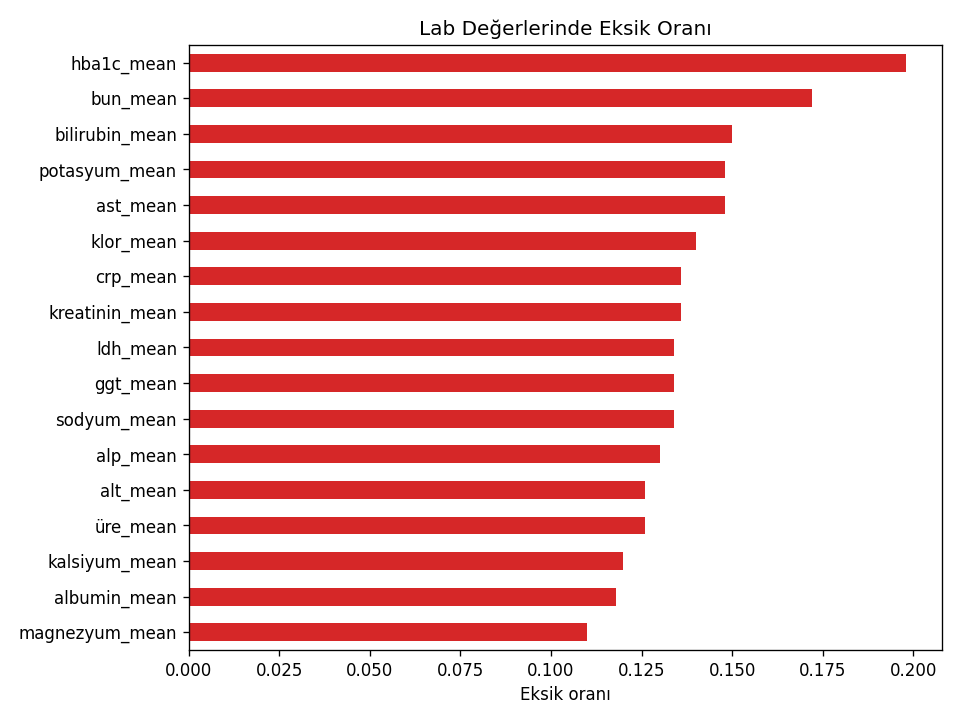
\includegraphics[width=7cm]{../figures/03_lab_missingness.png}
    \caption{Laboratuvar eksiklik oranları.}
\end{subfigure}\hfill
\begin{subfigure}[t]{0.46\textwidth}
    \centering
    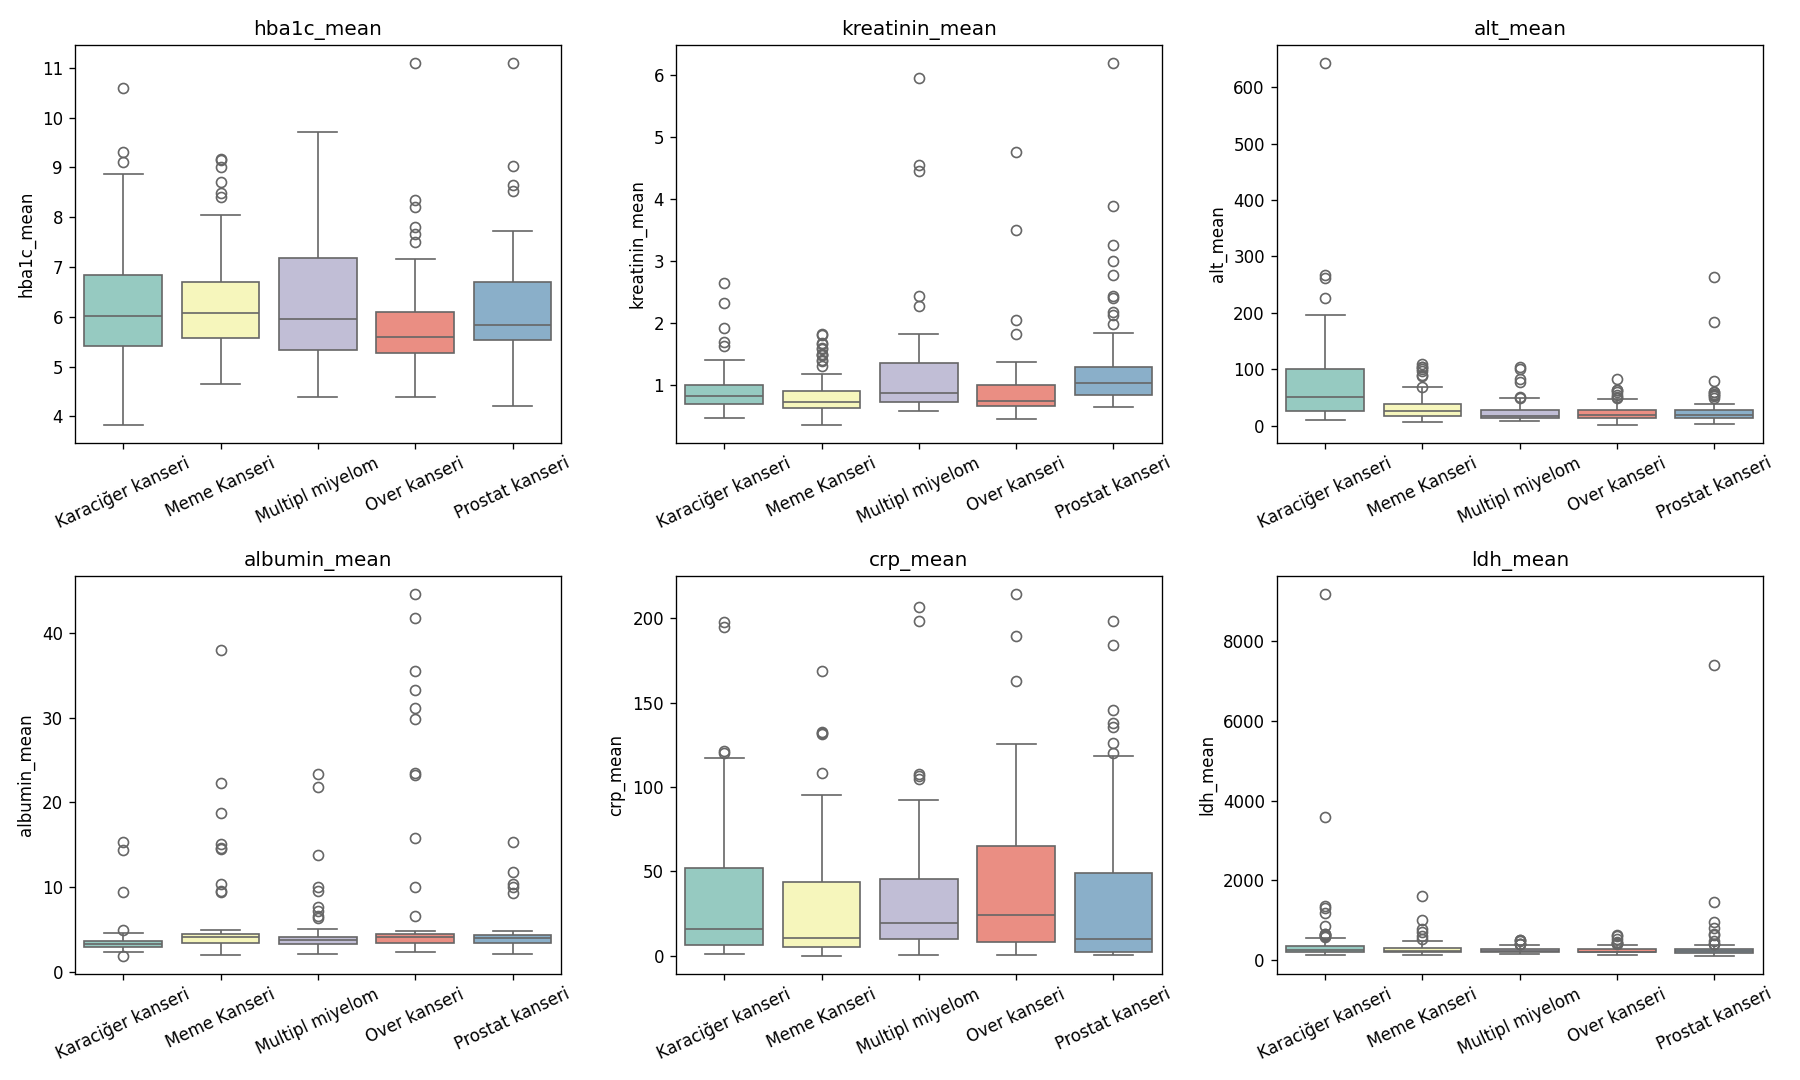
\includegraphics[width=7cm]{../figures/04_key_labs_by_cancer.png}
    \caption{Kilit laboratuvar değerleri.}
\end{subfigure}
\caption{Keşifsel veri analizi: demografi, eksiklik ve kanser türüne göre temel laboratuvar dağılımları.}
\label{fig:eda}
\end{figure}

Beklendiği üzere meme ve over kanseri kadın, prostat kanseri ise erkek hastalardan oluşmaktadır; karaciğer kanseri ve multipl miyelom her iki cinsiyette gözlenmektedir. Yaş dağılımında prostat kanseri (ortalama $75.2$) en yaşlı, over kanseri (ortalama $61.3$) en genç grubu oluşturmaktadır.

\FloatBarrier
\section{HbA1c Üzerinden Diyabet Yükü Analizi}

HbA1c, hem diyabet tanısı hem de uzun dönem glisemik kontrolün izlenmesinde kullanılan altın standart bir biyobelirteçtir. Amerikan Diyabet Derneği (ADA) eşiklerine göre değerler üç kategoriye ayrılır:
\begin{itemize}[leftmargin=2em,itemsep=0pt]
\item \textbf{Normal:} $\mathrm{HbA1c} < 5.7$
\item \textbf{Prediyabet:} $5.7 \leq \mathrm{HbA1c} < 6.5$
\item \textbf{Diyabet:} $\mathrm{HbA1c} \geq 6.5$
\end{itemize}

Her hasta için takip süresince ölçülen \emph{en yüksek} HbA1c değeri esas alınmıştır; bu, diyabet riskini tespit etmede daha duyarlı bir yaklaşımdır. Tablo~\ref{tab:hba1c} ve Şekil~\ref{fig:hba1c} sonuçları özetlemektedir.

\begin{table}[htbp]
\centering
\caption{Kanser türüne göre HbA1c kategorilerinin yüzde dağılımı.}
\label{tab:hba1c}
\small
\begin{tabular}{lcccc}
\toprule
\textbf{Kanser türü} & \textbf{Normal} & \textbf{Prediyabet} & \textbf{Diyabet} & \textbf{Bilinmiyor} \\
\midrule
Karaciğer kanseri   & \%25 & \%20 & \%34 & \%21 \\
Meme kanseri        & \%16 & \%32 & \%36 & \%16 \\
Multipl miyelom     & \%20 & \%17 & \%27 & \%36 \\
Over kanseri        & \%34 & \%31 & \%20 & \%15 \\
Prostat kanseri     & \%22 & \%28 & \textbf{\%39} & \%11 \\
\bottomrule
\end{tabular}
\end{table}

\begin{figure}[htbp]
\centering
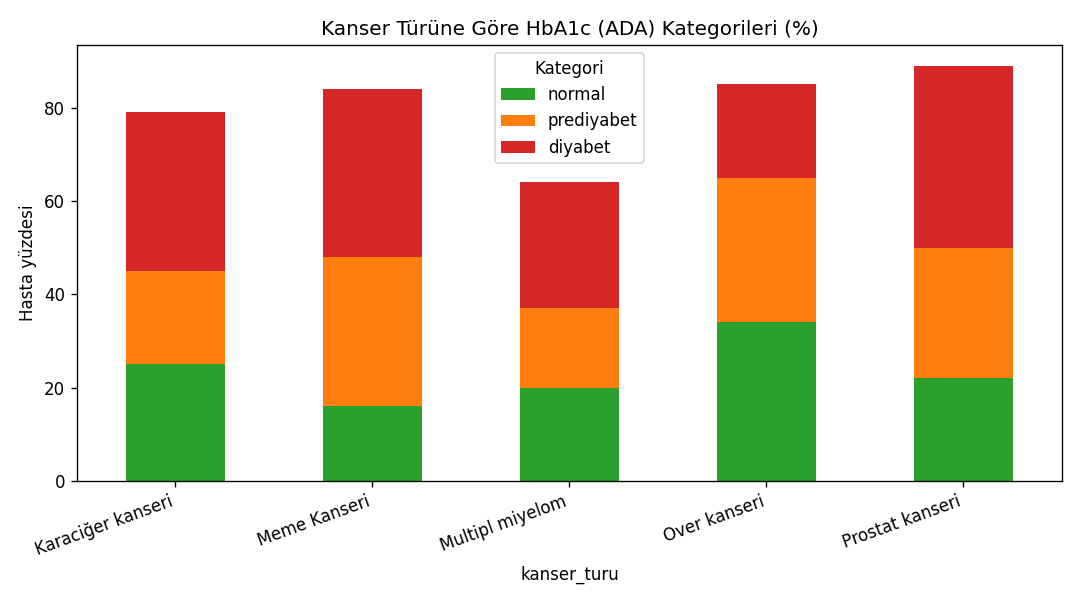
\includegraphics[width=11cm]{../figures/05_hba1c_categories.png}
\caption{Kanser türüne göre HbA1c kategorilerinin yığılı sütun grafiği (\%).}
\label{fig:hba1c}
\end{figure}

Beklenen ve gözlenen frekanslar üzerinde gerçekleştirilen Pearson ki-kare bağımsızlık testi, kanser türleri arasında HbA1c kategorilerinin dağılımında anlamlı bir farklılık olduğunu ortaya koymuştur:
\[
\chi^2 = 17.03,\quad \mathrm{dof} = 8,\quad p = 0.030.
\]
Diyabet oranı en yüksek olan grup prostat kanseri (\%39) iken, over kanseri (\%20) en düşük orana sahiptir. Klinik perspektiften bu bulgu, prostat ve meme kanseri takibi yapan onkoloji birimlerinde rutin HbA1c tarama protokollerinin ve metabolik komorbidite yönetiminin önceliklendirilmesi gerektiğine işaret etmektedir.

\section{Türkçe Epikriz Üzerinde Doğal Dil İşleme}

Veri setindeki epikriz metni, klasik klinik dokümantasyon yapısında (yakınma, öykü, izlem, plan) yazılmış zengin bir bilgi kaynağıdır. İki tamamlayıcı NLP analizi gerçekleştirilmiştir.

\subsection{TF-IDF ile Kanser Türüne Özgü Anahtar Terimler}

Her kanser türünün tüm epikriz metinleri tek bir belge olarak birleştirilmiş ve $5$ belge üzerinde TF-IDF vektörleştirmesi yapılmıştır. Türkçeye özgü temel bir durdurma sözcüğü (\emph{stopword}) listesi tanımlanmış, en az üç harfli yalnızca harf içeren tokenlar dikkate alınmıştır. Sonuçlar, terimlerin klinik olarak anlamlı sinyaller verdiğini göstermiştir: prostat için \texttt{psma}, over için \texttt{markerleri}, miyelom için \texttt{kür} (kemoterapi siklusu) gibi terimler ilk sıralarda yer almıştır.

\subsection{Regex Tabanlı Semptom Çıkarımı}

On adet sık görülen onkolojik semptom için Türkçe morfolojik varyantları yakalayan düzenli ifadeler tanımlanmıştır (\emph{ağrı, bulantı, kusma, yorgunluk/halsizlik, ateş, iştahsızlık, kilo kaybı, nefes darlığı, kabızlık, ishal}). Şekil~\ref{fig:semptom}, semptom sıklıklarının kanser türüne göre dağılımını sunmaktadır.

\begin{figure}[htbp]
\centering
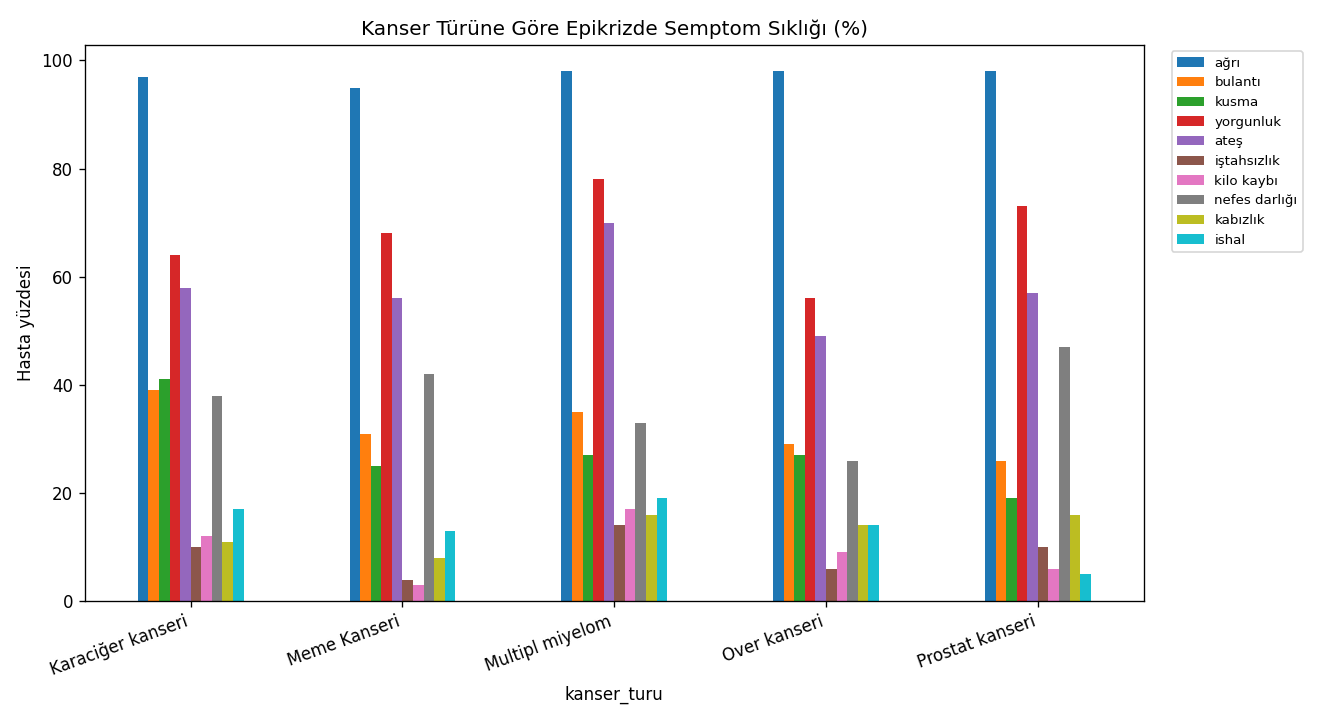
\includegraphics[width=14cm]{../figures/06_symptom_frequency.png}
\caption{Epikriz metinlerinde semptom yüzdeleri (kanser türüne göre).}
\label{fig:semptom}
\end{figure}

Tüm gruplarda \emph{ağrı} \%95'in üzerinde gözlenmiştir; bu, ileri evre onkoloji popülasyonu için beklenen bir bulgudur. Ayırt edici sonuçlar şunlardır: bulantı ve kusma karaciğer ile miyelom hastalarında daha yüksektir; nefes darlığı prostat (\%47) ve meme (\%42) kanserinde öne çıkmaktadır (kemik metastazı veya plevral efüzyon hipoteziyle uyumlu); kabızlık özellikle multipl miyelom ve prostat kanserinde belirgindir (opioid kullanımı ve hiperkalsemi olası nedenler arasındadır).

\FloatBarrier
\section{Baseline Sınıflandırıcılar}

Yalnızca rutin laboratuvar (\texttt{\_mean} özetleri), yaş ve cinsiyet özellikleriyle, beş sınıflı kanser türü tahmini görevinde iki baseline model değerlendirilmiştir. Eksik değerler medyan ile doldurulmuş, lojistik regresyon için ayrıca standart ölçeklendirme uygulanmıştır. Tüm değerlendirmeler, \texttt{random\_state=42} ile $5$-katlı tabakalı çapraz doğrulama (Stratified $K$-Fold) altında yapılmıştır.

\begin{table}[htbp]
\centering
\caption{$5$-katlı çapraz doğrulama performansı (rastgele $\approx$ \%20).}
\label{tab:model}
\small
\begin{tabular}{lcc}
\toprule
\textbf{Model} & \textbf{Doğruluk (ortalama $\pm$ s.s.)} & \textbf{Makro F1} \\
\midrule
Lojistik Regresyon & $0.684 \pm 0.027$ & $0.684$ \\
Rastgele Orman     & $\mathbf{0.712 \pm 0.031}$ & $\mathbf{0.710}$ \\
\bottomrule
\end{tabular}
\end{table}

Rastgele Orman, rastgele tahminin yaklaşık $3.5$ katı bir doğruluk elde etmiştir. Sınıf bazında en yüksek F1 skoru meme kanserinde ($0.90$) gözlenmiştir; bunun temel nedeni cinsiyet özelliğinin neredeyse tek başına meme kanserini diğer gruplardan ayırt etmesidir. En zor sınıf multipl miyelom (F1\,$=0.53$) olmuştur; karaciğer kanseri ile karışmaktadır, çünkü her iki grup da bozuk hepatik panel sergileyebilmektedir. Şekil~\ref{fig:cm_fi} hata matrislerini ve özellik önemlerini göstermektedir.

\begin{figure}[htbp]
\centering
\begin{subfigure}[t]{0.32\textwidth}
    \centering
    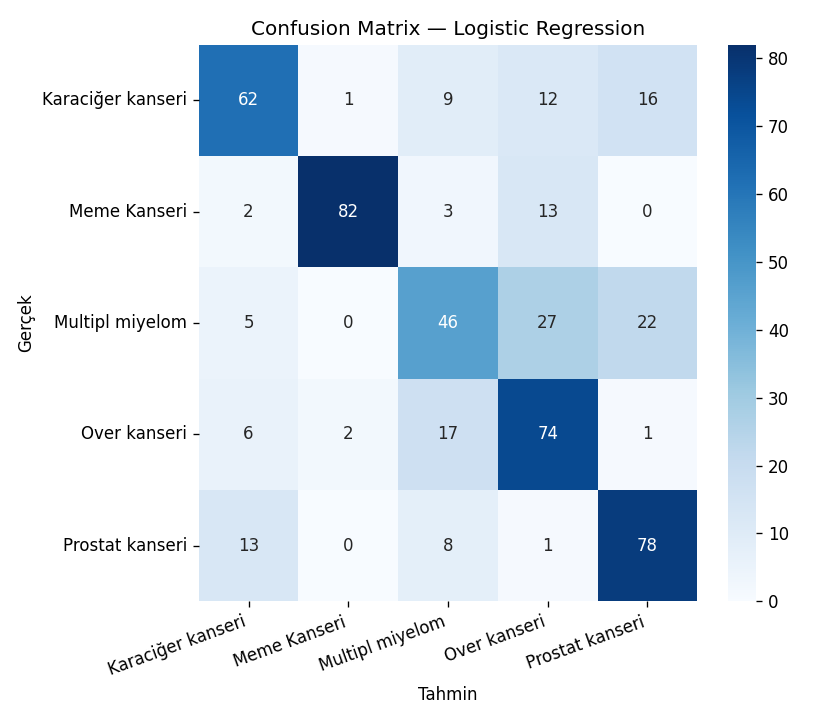
\includegraphics[width=4.8cm]{../figures/07_cm_logreg.png}
    \caption{Lojistik Regresyon.}
\end{subfigure}\hfill
\begin{subfigure}[t]{0.32\textwidth}
    \centering
    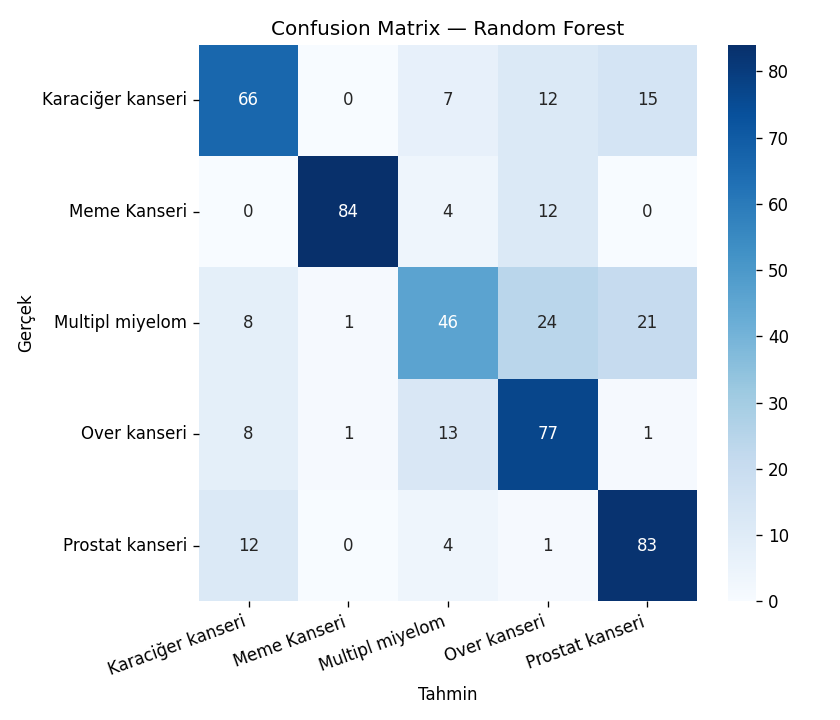
\includegraphics[width=4.8cm]{../figures/08_cm_rf.png}
    \caption{Rastgele Orman.}
\end{subfigure}\hfill
\begin{subfigure}[t]{0.32\textwidth}
    \centering
    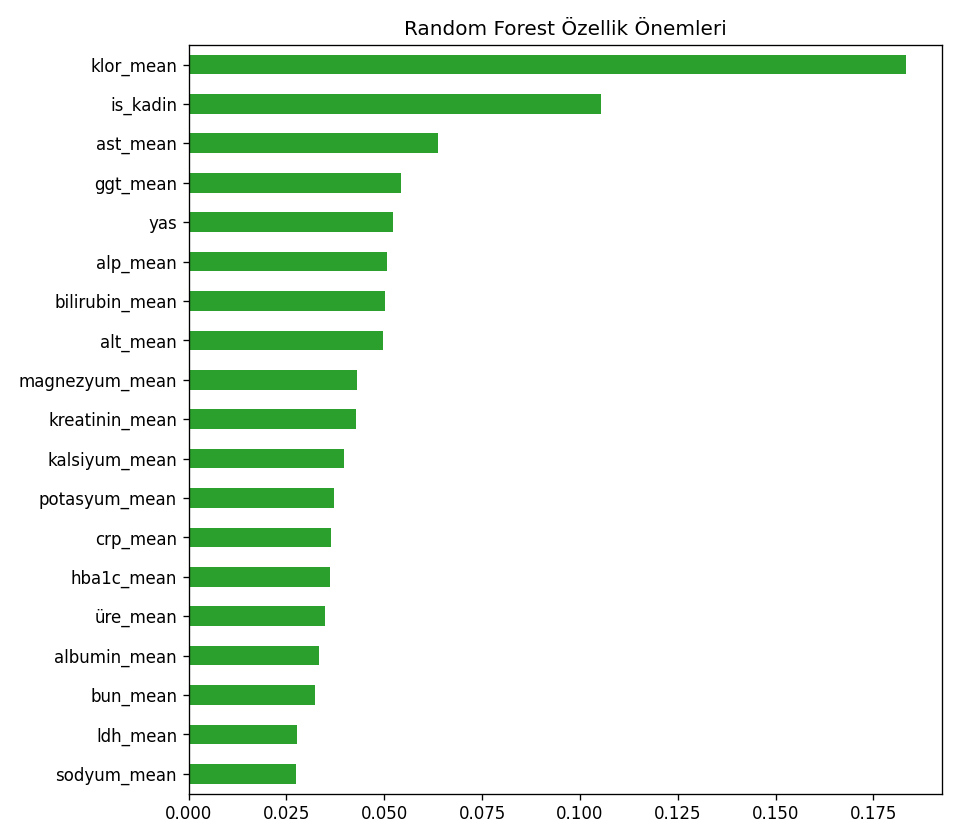
\includegraphics[width=4.8cm]{../figures/09_feature_importance.png}
    \caption{Özellik önemleri.}
\end{subfigure}
\caption{Modellerin hata matrisleri ve Rastgele Orman özellik önemleri.}
\label{fig:cm_fi}
\end{figure}

En önemli özellikler sırasıyla \emph{klor ortalaması, cinsiyet, AST, GGT} ve \emph{yaş} olarak bulunmuştur. Hepatobilier enzimlerin (AST, GGT) ön sıralarda yer alması, modelin biyolojik olarak anlamlı sinyalleri yakaladığının göstergesidir.

\FloatBarrier
\section{Klinik Uygulama Önerileri}

Bu basit baseline'lardan yola çıkarak şu uygulama fikirlerini önermekteyiz:

\begin{itemize}[leftmargin=1.5em,itemsep=1pt]
    \item \textbf{Otomatik metabolik tarama tetikleyicisi:} Prostat ve meme kanseri tanısı alan hastalar için elektronik hasta dosyasında HbA1c isteminin otomatik önerilmesi.
    \item \textbf{Türkçe semptom etiketleyici:} Epikriz girişi sırasında semptomları gerçek zamanlı olarak yapısal etiketlere çeviren ve standardizasyonu artıran bir NLP eklentisi.
    \item \textbf{Lab tutarlılık uyarı sistemi:} Mevcut tanı ile uyumsuz lab paterni durumunda klinisyene karar destek uyarısı veren bir modül.
\end{itemize}

\section{Sınırlamalar}

Çalışmanın temel sınırlamaları şunlardır: (i) örneklem $500$ hasta ile sınırlıdır ve veri setinde sentetik üretim izleri mevcut olabilir; (ii) lab değerleri zaman serisi içermesine rağmen yalnızca özet istatistikler kullanılmıştır; (iii) HbA1c için "Bilinmiyor" oranı (\%11--\%36) kanser türüne göre değişmektedir, bu da seçici olmayan veri eksikliği varsayımını ihlal edebilir; (iv) Türkçe NLP işleme minimal düzeyde tutulmuştur; üretim ortamında Zemberek veya BERTurk gibi morfolojik/sözcüksel kaynaklar kullanılmalıdır.

\section{Sonraki Adımlar}

\begin{enumerate}[leftmargin=1.5em,itemsep=1pt]
    \item Lab zaman serilerinden trend tabanlı özellikler (eğim, varyasyon) çıkarmak.
    \item Epikrizden BERTurk tabanlı varlık adı tanıma (NER) ile yapılı bilgi çıkarımı.
    \item \texttt{ölüm tarihi} sütunu üzerinden hayatta kalma analizi (Kaplan-Meier, Cox regresyonu).
    \item ATC kod hiyerarşisi kullanılarak ilaç temelli terapi profilleri ve kümeleme.
\end{enumerate}

\section{Tekrar Üretilebilirlik}

Tüm kod tabanı GitHub deposunda \texttt{stage1} dalında, on ayrı \emph{conventional commit} olarak yayımlanmıştır:
\begin{center}
\url{https://github.com/ahmeterdempmk/datamedx-hackathon-2}
\end{center}

Yeniden üretmek için:
\begin{verbatim}
pip install -r requirements.txt
python src/eda.py
python src/hba1c_analysis.py
python src/nlp_epikriz.py
python src/model_baseline.py
\end{verbatim}

\section*{Takım: CatBoost Baseline}

\begin{itemize}[leftmargin=1.5em,itemsep=1pt]
    \item \textbf{Ahmet Erdem Pamuk} (Kaptan) --- Mustafa Hakan Güvençer Fen Lisesi, Ankara \\ \texttt{ahmeterdempmkk@gmail.com}
    \item \textbf{Hamit Tuğrul Arslan} --- İstanbul Teknik Üniversitesi Mesleki ve Teknik Anadolu Lisesi, İstanbul
    \item \textbf{Ömer Kay} --- Özel Çağdaş Eğitim Anadolu Lisesi, İzmir
\end{itemize}

\end{document}
